\documentclass[xetex,mathserif,serif]{beamer}
\usepackage{polyglossia}
\setdefaultlanguage[babelshorthands=true]{russian}
\usepackage{minted}
\usepackage{tabu}
\usepackage{forest}
\usepackage{moresize}
\usepackage{textpos}

\useoutertheme{infolines}

\usepackage{fontspec}
\setmainfont{FreeSans}
\newfontfamily{\russianfonttt}{FreeSans}

\setbeamertemplate{blocks}[rounded][shadow=false]

\setbeamercolor*{block title alerted}{fg=red!50!black,bg=red!20}
\setbeamercolor*{block body alerted}{fg=black,bg=red!10}

\tabulinesep=1.2mm

\title{Веб-программирование}
\author[Юрий Литвинов]{Юрий Литвинов\\\small{\textcolor{gray}{yurii.litvinov@gmail.com}}}
\date{16.11.2017}

\newcommand{\todo}[1] {
	\begin{center}\textcolor{red}{TODO: #1}\end{center}
}

\newcommand{\DownArrow} {
	\hspace{2cm}\begin{LARGE}$\downarrow$\end{LARGE}
}

\newcommand{\attribution}[1] {
	\begin{flushright}\begin{scriptsize}\textcolor{gray}{#1}\end{scriptsize}\end{flushright}
}

\begin{document}

	\frame{\titlepage}

	\section{Введение}

	\begin{frame}
		\frametitle{Веб-приложения}
		\framesubtitle{Как оно вообще работает}
		\begin{itemize}
			\item Пользователь заходит браузером на определённый URL
			\begin{itemize}
				\item На самом деле, выполняя HTTP GET-запрос на порт 80 или 443 (обычно)
			\end{itemize}
			\item ОС сервера перенаправляет запрос запущенному там \textit{веб-серверу}
			\begin{itemize}
				\item Например, Apache, IIS
			\end{itemize}
			\item Веб-сервер --- отдельный процесс, в рамках которого запущено несколько \textit{веб-приложений}, веб-сервер по URL запроса определяет, какому веб-приложению он адресован, и передаёт запрос ему
			\item Веб-приложение формирует ответ и отправляет его обратно по HTTP в виде HTML-страницы
			\item Эта страница и показывается пользователю в браузере
		\end{itemize}
	\end{frame}

	\begin{frame}
		\frametitle{Веб-сервисы}
		\begin{itemize}
			\item \textit{Веб-сервис} --- это примерно то же самое, но не для пользователя, а для других приложений
			\item Нужны для создания распределённых приложений
			\item Общаются не с помощью HTML, а посредством специализированных протоколов
			\begin{itemize}
				\item Например, SOAP 
				\begin{itemize}
					\item Использует синтаксис XML, может использовать HTTP как транспорт
				\end{itemize}
			\end{itemize}
			\item Как правило, содержат механизм публикации метаинформации
			\begin{itemize}
				\item Например, WSDL
			\end{itemize}
			\item Реализуются посредством технологий, например, Windows Communication Foundation
		\end{itemize}
	\end{frame}

	\begin{frame}
		\frametitle{Веб-приложения и .NET}
		\begin{itemize}
			\item Веб-сервер --- IIS (Internet Information Services), IIS Express, Kestrel
			\begin{itemize}
				\item Есть ``из коробки'' в Windows, IIS Express поставляется с Visual Studio и используется для отладки
			\end{itemize}
			\item Технология для разработки веб-приложений --- ASP.NET MVC
			\begin{itemize}
				\item ASP.NET MVC 5
				\item ASP.NET MVC Core 2.0
			\end{itemize}
			\item Технология для разработки веб-сервисов --- WCF
			\item Работа с базами данных --- MS SQL Server (SQL Server Express)
			\item ORM --- Entity Framework (Entity Framework Core)
			\item Облачный хостинг --- Azure
		\end{itemize}
	\end{frame}

	\begin{frame}
		\frametitle{ASP.NET MVC, основные понятия}
		\begin{center}
			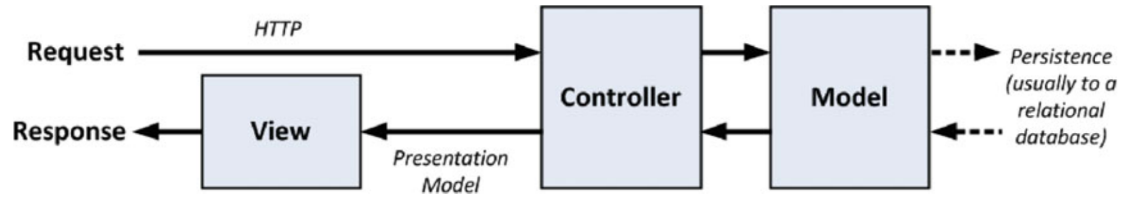
\includegraphics[width=0.7\textwidth]{mvc.png}
			\vspace{-5mm}
			\attribution{\textcopyright A. Freeman, Pro ASP.NET Core MVC}
		\end{center}

		\vspace{-5mm}

		\begin{itemize}
			\item \textbf{Модель} содержит или представляет данные, с которыми работает приложение
			\begin{itemize}
				\item \textbf{Domain model} содержит объекты предметной области вместе с бизнес-логикой, механизмами сериализации и т.д.
				\item \textbf{View Model} содержит классы, удобные для отображения во View, без бизнес-логики
			\end{itemize}
			\item \textbf{Представление} (View) отвечает за показ данных из модели пользователю
			\begin{itemize}
				\item Работает в браузере, но генерится на сервере
			\end{itemize}
			\item \textbf{Контроллер} отвечает за обработку входящих запросов, преобразование моделей и формирование данных для видов
		\end{itemize}
	\end{frame}

	\begin{frame}
		\frametitle{Работа с БД}
		\begin{itemize}
			\item Entity Framework
			\begin{itemize}
				\item Object-Relational Mapping-технология, представляет таблицы реляционной БД как объекты C\#
				\item Если вы пишете SQL руками в коде, вы делаете что-то не так
			\end{itemize}
			\item MS SQL Server LocalDB
			\begin{itemize}
				\item Реляционная СУБД, урезанная версия SQL Server, предназначенная прежде всего для разработчиков
				\item Не требует конфигурации, после установки экземпляр создаётся автоматически и к нему можно просто подключаться
			\end{itemize}
			\item На самом деле, подобных технологий только популярных десятки
			\begin{itemize}
				\item Например, MongoDB или SQLite неплохи
			\end{itemize}
		\end{itemize}
	\end{frame}

	\begin{frame}
		\frametitle{Entity Framework, подробности}
		\begin{itemize}
			\item Работа с базой делается через классы \textit{модели}
			\begin{itemize}
				\item Code first
				\item Database first
				\item Model first
			\end{itemize}
			\item \textit{DbContext} --- базовый класс, представляющий сессию при работе с базой
		\end{itemize}
	\end{frame}

	\begin{frame}[fragile]
		\frametitle{Немного примеров}
		\framesubtitle{Из \url{https://docs.microsoft.com/en-us/ef/core/}}
		\begin{tiny}
			Конфигурирование:
			\begin{minted}{csharp}
public class BloggingContext : DbContext
    {
        public DbSet<Blog> Blogs { get; set; }
        public DbSet<Post> Posts { get; set; }

        protected override void OnConfiguring(DbContextOptionsBuilder optionsBuilder)
        {
            optionsBuilder.UseSqlServer(@"Server=(localdb)\mssqllocaldb;Database=MyDatabase;Trusted_Connection=True;");
        }
    }
			\end{minted}
			Чтение:
			\begin{minted}{csharp}
using (var db = new BloggingContext())
{
    var blogs = db.Blogs
        .Where(b => b.Rating > 3)
        .OrderBy(b => b.Url)
        .ToList();
}
			\end{minted}
			Запись:
			\begin{minted}{csharp}
using (var db = new BloggingContext())
{
    var blog = new Blog { Url = "http://sample.com" };
    db.Blogs.Add(blog);
    db.SaveChanges();
}
			\end{minted}
		\end{tiny}
	\end{frame}

\end{document}
